% CHAPTER 3 (probably)
% Isoprene Emissions

\chapter{Isoprene Emissions in Australia} % Main chapter title
\label{ch_isop}

\section{GEOS-Chem isoprene mechanisms}
\label{ch_isop:sec:GEOSChemMechanisms}
  \subsection{Outline}
    The isoprene reactions simulated by GEOS-Chem were originally based on \cite{Horowitz1998}.
    This involved simulating NO$_X$, O$_3$, and NMHC chemistry in the troposphere at continental scale in three dimensions, with detailed NMHC chemistry with isoprene reactions and products.
    The mechanism was subsequently updated by \citet{Mao2013}, who change the isoprene nitrates yields and add products based on current understanding as laid out in \citet{Paulot2009a,Paulot2009b}.
    Further mechanistic properties, like isomerisation rates, are based on results from four publications: cite{Crounse2011,Crounse2012,Peeters2010,Peeters2011}.
    (TODO: check abstracts Peeters papers).
    \cite{Crounse2011} examines the isomerisations associated with the oxidation of isoprene to six different isomers (ISO$_2$) formed in the presence of oxygen: isoprene $ + OH \rightarrow^{O_2} $ ISO$_2$.
    They determine rates and uncertainties involved in these reactions, and study the rate of formation of C$_5$-hydroperoxyaldehydes (HPALDs) by isomerisation.
    \cite{Crounse2012} examine the fate of methacrolein (MACR), one of the products of isoprene oxidation. 
    Prior to this work MACR oxidation chamber studies were performed in high NO or HO$_2$ concentrations, giving peroxy lifetimes of less than 0.1~s.
    In most environments this is not the case, and MACR products over various NO concentrations and peroxy radical lifetimes are determined in their work.
    \cite{Peeters2010} examine photolysis of hydroperoxy-methyl-butenals (HPALDs, produced by isoprene isomerisation), which regenerates OH levels in areas with high isoprene emissions.
    Additionally, photolysis of photolabile peroxy-acid-aldehydes creates OH and improved model aggreement with continental observations.
   The OH and HPALD interactions are central to maintaining the OH levels in pristine and moderately polluted environments, which makes isoprene both a source and a sink of OH TODO: cite and DL;\url{http://www.nature.com/ngeo/journal/v5/n3/full/ngeo1405.html}.
    
    Formation of isoprene nitrates have an effect on ozone levels through NO$_X$ sequestration, and the yields and destinies of these nitrates is analysed in \citet{Paulot2009a}. 
    They use anion chemical ionization mass spectrometry (CIMS) to determine products of isoprene photooxidation.
    In a chamber with clean air and high NO concentrations, isoprene photooxidation is initially driven by OH addition, followed by NO$_X$ chemistry (150~min - 600~min), and finally HO$_X$ dominated chemistry.
    The yields of various positional isomers of isoprene nitrates is estimated, and pathways of their oxidation products is shown and used in the GEOS-Chem isoprene mechanism \citep{Paulot2009a,Mao2013}. 
    
    In low NO$_X$ conditions, isoprene oxidises to yield 70\% hydroxyhydroperoxides (ISOPOOH), which then oxidises to create dihydroxyperoxides (IEPOX) with OH recycling maintaining the OH levels in the atmosphere \citep{Paulot2009b}.
    In older models isoprene produced ISOPOOH which then titrated OH, however, the loss of OH has not been seen in measurements \citep{Paulot2009b,Mao2013}.
    The isoprene mechanism in GEOS-Chem has been updated to include OH regeneration from oxidation of epoxydiols and slow isomerisation of ISOPO$_2$ \citep{Mao2013}.
    
    Under high NO$_X$ conditions, isoprene undergoes OH addition at the 1 and 4 positions, becoming $\beta$ (71\%) or $\delta$ (29\%) hydroxyl peroxy radicals (ISOPO$_2$). 
    The $\beta$-hydroxyl reacts with NO$_X$ and produces HCHO (66\%), methylvinylketone (40\%) (MVK), methacrolein (26\%), and $\beta$-hydroxyl nitrates (6.7\%) (ISOPNB).
    The $\delta$-hydroxyl reacts with NO to form $\delta$-hydroxyl nitrates (24\%) (ISOPND), and ISOPNB (6.7\%).
    ISOPNB and ISOPND yield first generation isoprene at 4.7\% and 7\% respectively.
    
    Under low NO$_X$ conditions, ISOPO$_2$ may react with HO$_2$ to form ISOPOOH.
    In this case there is also production of HCHO (4.7\%), MVK(7.3\%), and MACR (12\%).
    As stated in earlier; most ISOPOOH will form IEPOX (epoxydiols) after reacting with OH and lead to OH regeneration.
    The other mechanism in low NO$_X$ environments is unimolecular isomerisation of ISOPO$_2$.
    This leads to production of hydroperoxyaldehydes (HPALDS), which generally photolyse and have an OH yield of 100\%.
    \citet{Mao2013} show that a lower (factor of 50) rate constant for ISOPO$_2$ isomerisation leads to better organic nitrate aggreements with ICARTT. 
    
    This update leads to more accurate modelling of OH concentrations, especially in low NO$_X$ conditions common in remote forests.
    Prior to \citet{Mao2012}, measurements of OH in high VOC regions may have been up to double the real atmospheric OH levels, due to formation of OH inside the instrument.
    \citet{Mao2012} examine an upgraded method of measurement, and compare these against a regional atmospheric chemistry model (RACM2), with the OH recycling updates from \citet{Paulot2009b} as discussed in prior paragraphs.
    
    The updates to isoprene chemistry by \citet{Mao2013}, and those shown in \cite{Crounse2011,Crounse2012} are the last before version 11, which was not used in this work.

    The full current mechanism is described online at \url{http://wiki.seas.harvard.edu/geos-chem/index.php/New_isoprene_scheme}.
    
  \subsection{Emissions from MEGAN}
    MEGAN simulates biogenic emissions of various gases including isoprene, based on various meteorological, land cover, and plant type parameterisations.
    
    One of the important parameters in Australia is the soil moisture activity factor($\gamma_{SM}$), which can have large regional affects on the isoprene emissions \citep{Sindelarova2014,Bauwens2016}.
    Generally if soil moisture is too low, isoprene emissions stop \citep{Pegoraro2004,Niinemets2010}, however in many Australian regions the plants may be more adapted to lower moisture levels. (TODO: Find cites for this - talk from K Emerson at Stanley indicated this)
    GEOS-Chem runs MEGANv2.1, which has three possible states for isoprene emissions based on the soil moisture ($\theta$):
    \begin{align*}
      \gamma_\mathrm{SM} & = 1 && \theta > \theta_1 \\
      \gamma_\mathrm{SM} & = (\theta-\theta_w)/\Delta\theta_1  && \theta_w < \theta < \theta_1 \\
      \gamma_\mathrm{SM} & = 0 && \theta < \theta_w \\
    \end{align*}
    where $\theta_w$ is the wilting point, and $\theta_1$ determines when plants are near the wilting point.
    The wilting point is set by a land based database from \citet{Chen2001}, while $\theta_1$ is set globally based on \citet{Pegoraro2004}.
    
    In GEOS-Chem the emissionscan be globally multiplied by a constant factor, which was performed to determine the smearing and sensitivity.
    By running the model two extra times, with the biogenic emissions set to zero and one half, while other parameters remain unchanged, the general affects of isoprene emissions which the model undergoes can be determined.
    
%----------------------------------------------------------------------------------------
%	SECTION
%----------------------------------------------------------------------------------------
\section{Isoprene emissions estimation}
\label{ch_isop:sec:IsopreneEmissions}

  \subsection{Outline}
   With the vertical columns of biogenic HCHO we can infer the local (grid space) isoprene emissions using effective molar formaldehyde yield (In other continents around 2-3, or 1 in low NO$_X$ conditions) \citep{Palmer2003,Marais2012,Bauwens2016}.
    If we assume there is fast HCHO yield, so that the effect of chemical transport is minimal, and that HCHO and isoprene are at steady states, then we can calculate local yield from our CTM.
    %This yield is derived from both HCHO and isoprene, such as was used by \citet{Millet2006} who produced a molar HCHO yield of 2.3 in north eastern USA.
   Yield is calculated from the modelled slope between isoprene emissions and HCHO total column within each gridbox over Australia, as performed in \cite{Palmer2003}, using modelled values between 1300-1400 LT which is around the overpass time of the OMI.
   This modelled yield is then used in conjunction with the recalculated OMI measurements in order to estimate isoprene emissions.
    
    The calculations used to determine isoprene emissions over Australia are fully described in \ref{ch_isop:sec:EmissionCalculation} and follow the method of \citet{Palmer2003}.
    To calculate emissions we use a reduced major axis (RMA) regression between modelled average (from 1300-1400 LT) values of the loss rates and total columns, an example is shown in figure TODO: figure with RMA of these over whatever time and space I end up using.
    
    The measured background HCHO is the average concentration measured in the remote pacific at the same time.
    The modelled background is determined from a run with isoprene emissions turned off, which allows us to see exactly how much the modelled isoprene emissions alter each vertical column of HCHO.
    
    Isoprene quickly forms HCHO in the atmosphere when in the presence of high levels of NO$_X$.
    However, over Australia NO$_X$ levels are generally not high enough and we must take extra care that we can account for the transport or 'smearing' caused by slower HCHO formation.
    Smearing sensitive grid boxes within the model can be detected by running the model with two uniformly differing isoprene emission levels, then finding the grid boxes where the changed HCHO column is greater than can be attributed to local emission difference.
    Using equation \ref{ch_isop:eqn:isop_yield} with two different isoprene emission levels:
    \begin{equation*}
      \hat{S} = \frac{\Delta~\Omega_{HCHO}}{\Delta~E_{ISOP}}
    \end{equation*}
    Consider halving the isoprene emitted globally and rerunning the model, if the local grid HCHO is reduced by much more than half (factoring yield) then you can infer sensitivity to non-local isoprene emissions.
    This can be dependent on local or regional weather patterns, as greater wind speeds will reduce the time any emitted compound stays within the local grid box.
    As such smearing sensitivity is both spatially and temporally diverse, shown in figure TODO: is a picture of the smearing sensitivity over Australia.
   
    Once the smearing sensitive grid squares are filtered out, application of equation \ref{ch_isop:eqn:isop_yield} gives us an estimate of isoprene emissions across the nation.
    
    Most recently a \citet{Bauwens2016} undertook a similar process to what I am doing, although with slightly different focus, using the IMAGESv2 global CTM instead of GEOS-Chem.
    They calculate emissions which create the closest match between model and satellite vertical columns, and compare these postiori data with the apriori (satellite data) and independent data sets.
    (TODO: simple outline of what they did and how my focus is different, this paper will also need to be summarised in the LitReview)

  \subsection{HCHO Products and yield}
    Australian forests are strong emitters of both isoprene and monoterpenes, which go on to form various products including secondary organic aerosols, oxygenated VOCs (OVOCs), ozone, OH, and HO$_2$.
    This production occurs over several steps, yields are often classed into at least two categories.
    First generation yield refers to the amount of HCHO produced per unit isoprene consumed by initial oxidation, total yield (sometimes molar yield) refers to time dependent yield of HCHO over multiple oxidation stages \citep{Wolfe2016}.
    \citet{Wolfe2016} define prompt yield as the change in formaldehyde measurement per unit change in initial isoprene emissions.
    Some argue that isoprene emissions are overestimated, due to the fact that they are based on relatively few measurements of isoprene emission factors \citep{Winters2009, FortemsCheiney2012} TODO: read and cite paper mentioned in Fortems.
    Recently \cite{Emmerson2017} showed that MEGAN estimates 3-6 times too much isoprene emissions, and 4 times too little monoterpenes when compared against 4 relatively small scale measurement campaigns in southeastern Australia.
    
    Isoprene production of HCHO depends on several factors, importantly NO$_X$ levels have a direct effect on the fate of VOCs in the atmosphere.
    At higher NO mixing ratios (at least a few hundred pptv), organic peroxy radicals (RO$_2$) react mostly with NO. 
    At low NO (less than 10's of pptv), reaction with HO$_2$, other RO$_2$, and isomerization dominate the fate of RO$_2$.
    In low NO$_X$ environments, reported HCHO yields from isoprene are from XtoY\%, while in high NO$_X$ environments this value is XtoY\% TODO: these values from table.
    For monoterpenes the yields are around X, Y\% for low, high NO$_X$ respectively.
    Emissions and yields for various species including some terpenes can be seen in table \ref{ch_isop:tab:VOCAusYields}.
    \citet{Wolfe2016} determine that going from NO$_X = 0.1$ to $2.0$ ppbv triples the prompt yield of HCHO, from 0.3 to 0.9 ppbv ppbv$^{-1}$ due to isoprene, while the background HCHO doubles.
    They determine prompt yield as the change in HCHO per change in ISOP$_0$, using $[ISOP]_0=[ISOP]\exp(k_1[\mathrm{OH}]t)$; where $k_1$ is first order loss rate.
    This effectively relates HCHO abundance with isoprene emission strength.
    (TODO:and finish Wolfe2016 discussion paper for yields)
    TODO:go through atkinsonarey2003
    
    Many of the HCHO yields from terpenoids are estimated through chamber studies which examine the products molecular mass and charge after mixing the compound of choice into a known volume of air.
    These conditions generally don't match those of the real world, where ambient air will have a cocktail of these compounds as well as various reactants.
    
    A proton transfer reaction mass spectrometer (PTR-MS) can be used to determine gas phase evolution of terpene oxidation products.
    This is done through analysis of mass to charge ratios ($m/z$) which can be used identify chemical compounds.
    Looking at Australian emissions from running GEOS-Chem and using yields provided by XYZ (TODO other table), we see that Australia may be more or less likely to do something TODO: this comparison sentence would be good to tie up tables and be copied to conclusions.
    
    Conversions between HCHO per unit C yield and molar \% yield from species X given by the equation $ Y_{molar \%} = 100 \times C_X \times Y_{HCHO per unit C} $, where $C_X$ is how many Carbon are within species X (5 for isoprene, 10 for monoterpenes, etc...).
    For instance a 200\% molar yield of HCHO from isoprene implies 1 Mole of C$_5$H$_8$ becomes 2 Mole HCHO which is a 0.4 HCHO per unit C yield.
    
    TODO: Fill out this table
    \begin{table} \begin{threeparttable}
      \caption{HCHO yields from various species averaged over Australia during Summer.}
      \begin{tabular}{ | c  c  c  c  c | }
        \toprule
	  \textbf{Species}   & \textbf{Emissions$^a$}& \textbf{Lifetime$^b$}& \textbf{HCHO Yield$^c$} & \textbf{HCHO production$^d$\%}
	  \\                 & (Tg C per month)      &                      & (per C reacted)         &         \\
	\midrule
	  Isoprene           & Y                     & n minutes            & 0.x                     & 10       \\
	  $\alpha$-Pinene    & Y                     & n minutes            & 0.x                     & 10       \\
	  $\beta$-Pinene     & Y                     & n minutes            & 0.x                     & 10       \\
	  HCHO               & Y                     & n minutes            & 1.0                     & 10       \\
	\bottomrule
      \end{tabular}
      \begin{tablenotes} 
	  \item a: Calculated using GEOS-Chem emissions over Australia in January 2005.
	  \item b:  
	  \item c: 
	  \item d: Production determined by dividing emission*yield by the sum of all VOC emissions*yields. 
      \end{tablenotes}
      \label{ch_isop:tab:VOCAusYields}
    \end{threeparttable} \end{table}
    
    % yields from Atkinsen2003
    %isoprene
    %0.63 0.10 Tuazon and Atkinson (1990a)
    %0.57 0.06 Miyoshi et al. (1994)
    % a-pinene
    %0.23 0.09 Noziere et al. (1999a)
    %0.19 0.05 Orlando et al. (2000)
    % b-pinene
    %0.54 0.05 Hatakeyama et al. (1991)
    %0.45 0.08 Orlando et al. (2000)
    
    Yields table looking at literature provided yields of HCHO.
    % molar HCHO yield per unit carbon equal to HCHO molar percent yield(per carbon)? or some conversion?
    % TODO: ask steve about ppbv ppbv^-1 ??
    
    \begin{table} \begin{threeparttable}
      \caption{ HCHO yields from various species, and lifetime against oxidation by OH. }
      \begin{tabular}{  l  l  l  l  l  }
        \toprule
        Species    & HCHO Yield      & Life vs OH & NO$_X$ background & Source   \\
                   & (molar \% )     &            &                   &          \\
      	\midrule 
      	Isoprene	& 315$\pm$50      &              & High           & a        \\ 
      			& 285$\pm$30      &        & High               & a        \\ 
      			& 225             & 35 min & High               & b        \\ % Done
      			& 150             &            & Low                & b        \\ % Done
      			& 150             &            & Low                & d        \\
      			& 450             &            & High               & d        \\
			& 235             &            & 1~ppbv              & e        \\
			& 150             &            & 0.1~ppbv              & e        \\
	$\alpha$-Pinene & 28$\pm$3        &        & Low                & c        \\ 
			& X$\pm$3         &        & X                  & d        \\ 
      			& 230$\pm$90      &        & High        & a        \\ 
      			& 190$\pm$50      &        & High        & a        \\ 
      			& 19                & 1 hour &              & b        \\ % Done
                      & 210               &          & 1~ppbv              & e        \\
                      & 70                &          & 0.1~ppbv              & e        \\
	$\beta$-Pinene    & 65$\pm$6        &        & Low                & c      \\ 
      			          & X$\pm$3         &        & X                  & d      \\ 
      			          & 540$\pm$50      &        & High               & a     \\ 
      			          & 450$\pm$80      &        & High               & a      \\ 
      			          & 45              & 40 min &              & b      \\ % Done
	Methane 	      & 100             & 1 year  &             & b     \\ 
	Ethane            & 180             & 10 days &             & b     \\ 
	Propane           & 60              & 2 days  &             & b     \\ 
	Methylbutanol    & .13(per C)    & 1 hour  &             & b     \\ 
	HCHO             & 100             & 2 hour  &             & b     \\ 
	Acetone           & .67(per C)      & 10 days &             & b     \\ 
	Methanol          & 100             & 2 days  &             & b     \\ %Done
    	\bottomrule
    \end{tabular}
    \begin{tablenotes} % \item makes new lines
      \item a \citet{AtkinsonArey2003}: Table 2, Yield from Isoprene reaction with OH, two values are from two referenced papers therein.
      \item b \citet{Palmer2003}: lifetimes assume [OH] is 1e15 mol cm$^{-3}$.
      \item c \citep{Lee2006}: Calculated through change in concentration of parent and product linear least squares regression.
        Estimates assume 20$^\circ$~C conditions.
  	  \item d \citet{Wolfe2016}: ``prompt yield'': change in HCHO per change in ISOP$_0$.
  	    $[ISOP]_0=[ISOP]\exp(k_1[\mathrm{OH}]t)$; where $k_1$ is first order loss rate.
  	    Effectively relates HCHO abundance with isoprene emission strength
      \item e \citet{Dufour2009}: One-day yields from oxidation modelled by CHIMERE, using MCM reference scheme.
      \item f Calculated using PTR-MS and iWAS on SENEX campaign data.
    \end{tablenotes}
    \label{ch_isop:tab:VOCLiteratureYields}
  \end{threeparttable} \end{table}
    
  \subsection{CAABA/MECCA yield}
  \label{Ch_isop:sec:CAABAMECCA}
    CAABA/MECCA is described in \ref{ch_LitRev:sec:CAABAMECCAIntro}.
    
    Using CAABA/MECCA to examine isoprene to HCHO yield in specific scenarios allows us to determine what environment may be driving the yield calculated by GEOS-Chem.
    This software runs gas and aqueous phase, and heterogeneous chemistry, including basic HO$_X$, NO$_X$, and NMHC chemistry, with emission, deposition, and initial concentrations all set.
    By running the same simulation twice, and injecting a small amount of extra isoprene into one of the simulations, extra HCHO produced can be used to determine the yield from isoprene to HCHO.
    Isoprene life time can also be calculated using this process, as the time it takes for the extra isoprene to reach $1/e$ of it's initial value.
    
    Initially we have three scenarios, grassland, desert, and forest Australia - with each scenario having initial conditions, emission and deposition set as in table \ref{ch_isop:tab:CaabaMeccaScenarioYields}.
    Running each scenario with and without a small isoprene injection gives isoprene lifetimes and isoprene to HCHO yield for those scenarios, shown in table \ref{ch_isop:tab:CaabaMeccaScenarioYields}.
    Calculation of the yield follows a calculation of the theoretical maximum carbon production by the amount of injected isoprene:
    \begin{equation}
      Y_{100} =10^9 \times \frac{C_{PM} E_{inj} D_{inj}}{(N_A H_{PBL})}
    \end{equation}
    Where Y$_{100}$ is the maximum possible carbon yield of isoprene (ppb), $C_{PM}$ is Carbon per molecule (isoprene=5), $E_{inj}$ is the emission rate of injected isoprene (molec cm$^{-2}$ s$^{-1}$), $D_{inj}$ is the duration of injection (s), H$_{PBL}$ is the boundary layer height (cm), and $N_A$ is the Air number density (molec cm$^{-3} \approx 2.5e19$).
    Finding the accumulated increase in HCHO (ppb) from the difference between the perturbed and non perturbed model runs allows calculation of the accumulated extra HCHO (Example: Figure TODO:), which divided by the $Y_{100}$ gives us the isoprene to HCHO atom C yield:
    \begin{equation}
      Y_{HCHO}= \frac{\Delta HCHO_{\text{Accumulated}}}{Y_{100}}
    \end{equation}
    with $HCHO_{\text{Accumulated}}$ being the accumulated enhanced ppb mixing ratio of HCHO.
    
    TODO: Fill in table
    \begin{table}
    	\caption{Scenario isoprene yields of HCHO}
    	\begin{tabular}{ p{6cm} l  l  l  l }
    		\hline
    		\textbf{Scenario} & \textbf{Emission} & \textbf{NO$_X$} & \textbf{HO} & Yield \\
				    		  & (molecules units) & (units)         & (units)     & units \\ \hline
    		Forest 	& xx 	& xx 	& xx 	& xx  	\\ 
    		Urban 	& xx 	& xx 	& xx 	& xx 	\\
    		Shrub 	& xx 	& xx 	& xx 	& xx 	\\ \hline
    	\end{tabular}
    	\label{ch_isop:tab:CaabaMeccaScenarioYields}
    \end{table}
    
    Figure TODO: shows the accumulated yield for all three scenarios, which each increase towards a limiting value.
    
  \subsection{Calculation of Emissions}
    \label{ch_isop:sec:EmissionCalculation}
    As is done in \citet{Palmer2003, Millet2006, Bauwens2016}, we assume that HCHO, and Isoprene columns are in a steady state, with no horizontal transport.
    In these circumstances the emissions of precursors are easy to calculate as long as we know the molar HCHO yields (Y$_i$) and effective chemical loss rates (k$_i$):
    \begin{equation}
      \Omega_{HCHO} = \frac{1}{k_{HCHO}}\Sigma_i k_i Y_i \Omega_i = \frac{1}{k_{HCHO}}\Sigma_i Y_i E_i
    \end{equation}
    
    We can infer the local (grid space) isoprene emissions (E$_{isop}$) using effective formaldehyde yield from isoprene ($Y_{isop}$).
    \begin{equation} \label{ch_isop:eqn:isop_yield}
      \Omega_{HCHO} = S \times E_{isop} + B
    \end{equation}
    Where \textit{B} is the background HCHO, and $S = Y_{isop}/k_{HCHO}$ is determined monthly as the regression between $k_{HCHO}*\Omega_{HCHO}$, and $k_{isop}*\Omega_{isop}$.
    The other equivalent method determines S from the RMA regression between $\Omega_{HCHO}$ and E$_{isop}$ on daily saved outputs from GEOS-Chem over Australia using 2 by 2.5$^{\circ}$ horizontal resolution.
    For an initial estimate of the effective yield from simulated data: we use $k_{HCHO}$, $k_{i}$, $\Omega_{HCHO}$, and $\Omega_i$ outputs from a standard run of GEOS-Chem - which provides one data point per day.
    This gives us a value for $Y_i$ resolved to our 2$^{\circ}$ by 2.5$^{\circ}$ horizontal resolution, which is entirely based on the model, and can be compared against the yield calculated using OMI derived $\Omega_{HCHO}$.
    Using our measurements of the biogenic HCHO column ($\Omega_{OMIHCHO}$) recalculated from the OMI satellite product, we use this derived yield and the same formula to determine our new top-down emissions estimates.
    Figure \ref{ch_isop:fig:E_isop_vs_hcho_model_sample} shows the modelled isoprene emissions and column concentrations along with the RMA regression line, sampled from grid boxes over Australia for January 2005. 
    Some affects from the low emissions in grid boxes which are largely oceanic can be seen and are handled by TODO: handle these and document here.
    
    \begin{figure}[!htbp]
      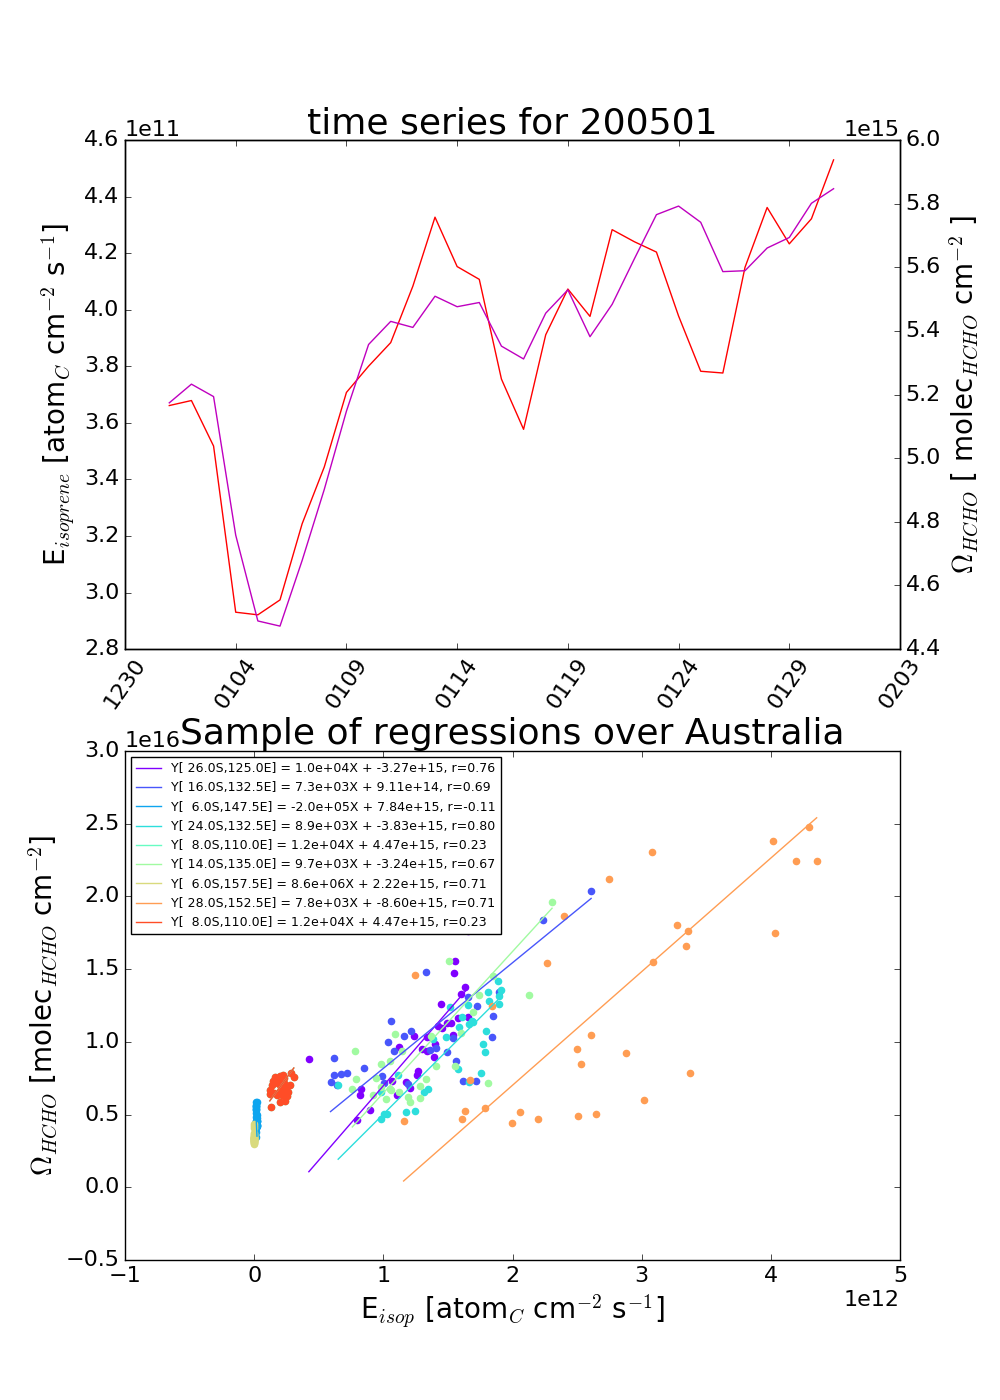
\includegraphics[width=\textwidth]{Figures/HCHO/GClink/E_isop_vs_hcho_series_200501.png}
      \caption{%
	Top panel: isoprene emissions for January, 2005, shown in red, coplotted with tropospheric hcho columns, shown in magenta.
	Both series are daily averages over Australia.
	Bottom panel: (RMA) linear regressions from between emissions of isoprene and tropospheric hcho columns, sampled randomly from the 2$^{\circ}$ by 2.5$^{\circ}$ latitude longitude gridboxes over Australia for the month of January (2005).
      }
      \label{ch_isop:fig:E_isop_vs_hcho_model_sample}
    \end{figure}
    
    This works if there is fast HCHO yield, so that the effect of chemical transport is minimal.
    The background HCHO is calculated using measurements in the remote pacific at the same time and latitude.
    Table \ref{ch_isop:tab:VOCAusYields} shows the average yield calculated for Australia. (TODO: this table and some notes)
    
  \subsection{Calculation of smearing effect}
    TODO: Smearing scale length, $\hat{S}$ formula, and results of calculations in here.
    As shown in \cite{Palmer2003}, smearing sensitivity can be calculated through multiple runs of the same model with the only difference being the isoprene emissions.
    I have run GEOS-Chem with and without E$_{ISOP}$ multiplied uniformly by 0.5, and the grid boxes with the most affected $\Omega_{HCHO}$ are those affected most by smearing.
    The smearing parameter  ($\hat{S}$) is defined as follows:
    \begin{equation}
      \hat{S} = \frac{\Delta \Omega_{HCHO}}{\Delta E_{ISOP}}
    \end{equation}
    TODO: Plot shows smearing parameter over Australia.
  
  \subsection{Calculations of uncertainty}
    There are several factors which need to be considered when looking at the uncertainty in emissions estimates.
    Things with their own inherent uncertainty include the modelled apriori, modelled relationship between HCHO and isoprene, and satellite measurements. 
    Important factors which need to be analysed for confidence in results include the steady state assumptions, filtering techniques for fire and human influences, and the regression model for determining the isoprene to HCHO yield.

    Uncertainty in satellite measurements is generally provided along with the data, although uncertainty introduced through AMF calculation needs to be determined to give a representation of the confidence in vertical column amounts.
    The measurement uncertainty is shown in section \ref{ch_HCHO:sec:OMI_uncertainty_calculation}, and amounts to $\sim X\%$. (TODO this number when calculated)
    
    Model uncertainty is difficult to accurately assertain, generally an analysis of the model compared to in-situ measurements is performed, however there are few of these measurements over Australia.
    TODO: find out how this is estimated in other papers, or else point to HCHO uncertainty and used some function of that.
    
    The uncertainty for HCHO to isoprene mechanisms TODO: how to do this?
  
  \subsection{Extrapolating the circadian cycle}
    Isoprene emissions occur with regular daily cycles caused by things like local temperature, sunlight, drought, and other environmental factors (TODO: find/cite eucalypt isoprene paper, daily cycle plot if can find).
    
    (TODO: following stuff, add some basic plots and error analysis eventually also)
    Using a model of the daily isoprene emissions fit to the offset determined by satellite HCHO based estimates, we produce a high temporal resolution isoprene emissions inventory.
    During days with more than one HCHO column measurement we can more confidently fit the cycle. 
    For example EOS AURA's OMI measurements from 2004 can be combined with MetOp-A's GOME2 after October 2006, with daily overpasses by OMI and GOME2 at 1345 and 0930 respectively.
    This allows a better retrieval of the daily amplitude of isoprene emissions.
    
  \subsection{Comparison with MEGAN}
    TODO: Direct comparison here, maps of differences for some metrics(monthly average,?). comparison of model run results using different inventory shown in section (reference here)

\section{New estimates affects on the Australian atmosphere}

